\chapter{A meta analysis of tournaments and an evaluation of performance in the
Iterated Prisoner's Dilemma.}\label{chapter:meta_tournaments}

\begin{center}
    The research reported in this Chapter has lead in a manuscript, entitled: \\
    \textbf{``Properties of winning Iterated Prisoner's Dilemma strategies''} \\
    Available at: \url{https://arxiv.org/abs/2001.05911} \\
    Associated data sets: \cite{Glynatsi2019_meta, Glynatsi2019_meta_raw_data} \\
    Axelrod-Python library version: 3.0.0 \\ \vspace{.5cm}
    The manuscript's abstract is the following:
\end{center}

Researchers have explored the performance of Iterated Prisoner's Dilemma strategies
for decades: from the celebrated performance of Tit for Tat, to the
introduction of the zero-determinant strategies, to the use of sophisticated learning
structures such as neural networks, many new strategies have been introduced and tested
in a variety of tournaments and population dynamics. Typical results in the literature,
however, rely on performance against a small number of somewhat arbitrarily selected
strategies in a small number of tournaments, casting doubt on the generalisability
of conclusions. We analyse a large collection of \numberofstrategies
strategies in \numberofalltournaments tournaments, present the top performing strategies across multiple
tournament types, and distill their salient features.
The results show that there is not yet a single
strategy that performs well in diverse Iterated Prisoner's Dilemma scenarios,
nevertheless there are several properties that heavily influence the best performing
strategies. This refines the properties described by R. Axelrod in light of
recent and more diverse opponent populations to: be nice, be provocable and generous,
be a little envious, be clever, and adapt to the environment. More precisely,
we find that strategies perform best when their probability of cooperation
matches the total tournament population's aggregate cooperation probabilities,
or a proportion thereof in the case of noisy and probabilistically ending tournaments,
and that the manner in which a strategy achieves the ideal cooperation rate is crucial.
The features of high performing strategies help cast some light on why strategies such as Tit For Tat
performed historically well in tournaments and why zero-determinant strategies
typically do not fare well in tournament settings.

\hrulefill

The differences between the Chapter and the manuscript include \dots.

\section{Introduction}

As stated in Chapter~\ref{chapter:introduction} conceptualising strategies and
understanding the best way of playing the game has been of interest to the
scientific community since the formulation of the game. In
Chapter~\ref{chapter:literature_review} it was established that following the
computer tournaments of Axelrod in the 1980's, a strategy's performance in a
round robin computer tournament became a common evaluation technique for newly
designed strategies. A large collection of works were discussed in
Chapter~\ref{chapter:literature_review} which introduced a broad collection of
strategies, and new strategies and competitions are published frequently,
as established in Chapter~\ref{chapter:bibliometric_study}. The question,
however, still remains the same: what is the best way to play the game?

Compared to the works reviewed in Chapter~\ref{chapter:literature_review}, where
typically a few selected or introduced strategies are evaluated on a small
number of tournaments and/or small number of opponents, this Chapter evaluates
the performance of \numberofstrategies strategies in \numberofalltournaments
tournaments. Furthermore, a large portion of these strategies are drawn from the
known and named strategies in IPD literature, including many previous tournament
winners, in contrast to other work that may have randomly generated many
essentially arbitrary strategies (typically restrained to a class such as
memory-one strategies, or those of a certain structural form such as finite
state machines or deterministic memory two strategies). Additionally, the
analysis of this Chapter considers tournament variations including standard
tournaments, tournaments with noise, probabilistic match length, and both noise
and probabilistic match length. This diversity of strategies and tournament
types yields new insights and tests earlier claims in alternative settings
against known powerful strategies.

The later part of the Chapter evaluates the impact of features on the
performance of the strategies using modern machine learning techniques. These
features include measures regarding a strategy's behaviour as well as measures
regarding the tournaments. The outcomes reinforce the discussion started by
Axelrod on properties of successful strategies (as presented in
section~\ref{section:intelligent_design}), and conclude that the properties are:

\begin{itemize}
    \item \st{Do not be envious} Be a little bit envious
    \item Be ``nice'' in non-noisy environments or when game lengths are longer
    \item Reciprocate both cooperation and defection appropriately;
    Be provocable in tournaments with short matches, and generous when matches are longer
    \item \st{Do not be too clever} It is okay to be clever
    \item Adapt to the environment; Adjust to the mean population cooperation
\end{itemize}

The rest of the Chapter is structured as follows:

\begin{itemize}
    \item section~\ref{section:data_collection} covers the different tournament
    types and the data collection which are made possible due to APL.
    \item section~\ref{section:top_performances} focuses on the best performing
    strategies for each type of tournament and overall.
    \item section~\ref{section:evaluation_of_performance}, explores the traits
    which contribute to a good performance.
\end{itemize}

\section{Data collection}\label{section:data_collection}

The data set generated for this Chapter was created with APL version 3.0.0.
APL allows for different types of IPD computer
tournaments to be simulated and contains a large list of strategies.
Most of these are strategies described in the literature with a few exceptions
of strategies that have been contributed specifically to the package. A
list of the strategies is given in the Appendix~\ref{app:list_of_players}.
Although APL features several tournament types, only
standard, noisy, probabilistic ending, and noisy probabilistic ending
tournaments are considered here.

\textit{Standard tournaments} are tournaments similar to that of Axelrod's
tournaments~\cite{Axelrod1980a}. There are \(N\) strategies which all play an iterated
game of \(n\) number of turns against each other. Note that self-interactions
are not included. Similarly, \textit{noisy
tournaments} have \(N\) strategies and \(n\) number of turns, but at each turn
there is a probability \(p_n\) that a player's action will be flipped.
\textit{Probabilistic ending tournaments}, are of size \(N\) and after each turn
a match between strategies ends with a given probability \(p_e\). Finally,
\textit{noisy probabilistic ending} tournaments have both a noise probability
\(p_n\) and an ending probability \(p_e\). For smoothing the simulated results a
tournament is repeated for \(k\) number of times. This was allowed to vary
in order to evaluate the effect of smoothing. The winner of each tournament
is based on the median score a strategy achieved and not by the number of wins.

The process of collecting tournament results is described by
Algorithm~\ref{algorithm:data_generation}. For each trial a random size \(N\) is
selected, and from the \numberofstrategies strategies a random list of \(N\) strategies is
chosen. For the given list of strategies a standard, a noisy, a probabilistic
ending and a noisy probabilistic ending tournament are performed and repeated
\(k\) times. The parameters for the tournaments, as well as the number of
repetitions, are selected once for each trial. The parameters and their
respective minimum and maximum values are given by
Table~\ref{table:parameters_values}.

\begin{table}[!htbp]
    \begin{center}
        \resizebox{.6\textwidth}{!}{
        \begin{tabular}{lcccc}
    \toprule
    parameter & parameter explanation &   min value & max value \\
    \midrule
    $N$ & number of strategies  & 3 & 195 \\
    $k$ & number of repetitions  & 10 & 100 \\
    $n$ & number of turns      & 1 & 200 \\
    $p_n$ & probability of flipping action at each turn  & 0 & 1   \\
    $p_e$ & probability of match ending in the next turn & 0 & 1   \\
    \bottomrule
        \end{tabular}}
    \end{center}
    \caption{Data collection; parameters' values}
    \label{table:parameters_values}
\end{table}

\begin{algorithm}[!htbp]
    \setstretch{1.35}
    \ForEach{\text{seed} $\in [0, 11420]$}{
        $N \gets \text{randomly select integer}\in [N_{min}, N_{max}]$\;
        $\text{players} \gets  \text{randomly select $N$ players}$\;
        $k \gets  \text{randomly select integer}\in [k_{min}, k_{max}]$\;
        $n \gets  \text{randomly select integer}\in [n_{min}, n_{max}]$\;
        $p_n \gets  \text{randomly select float}\in [p_{n\, min}, p_{n\, max}]$\;
        $p_e \gets   \text{randomly select float}\in [p_{e\, min}, p_{e\, max}]$\;
        \vspace{0.4cm}
        $\text{result standard}$ $\gets$ Axelrod.tournament$(\text{players}, n, k)$\;
        $\text{result noisy}$ $\gets$ Axelrod.tournament$(\text{players}, n, p_n, k)$\;
        $\text{result probabilistic ending}$ $\gets$ Axelrod.tournament$(\text{players}, p_e, k)$\;
        $\text{result noisy probabilistic ending}$ $\gets$ Axelrod.tournament$(\text{players}, p_n, p_e, k)$\;

    }
    \KwRet{result standard, result noisy, result probabilistic ending,
    result noisy probabilistic ending}\;
    \caption{Data collection Algorithm}
    \label{algorithm:data_generation}
\end{algorithm}

A total of \uniquenumberofseeds trials of Algorithm~\ref{algorithm:data_generation} have been
run. For each trial the results for 4 different tournaments were collected,
thus a total of \numberofalltournaments $(\uniquenumberofseeds \times 4)$ tournament results have been
retrieved. Each tournament outputs a result summary in the form of
Table~\ref{table:output_result}. Each strategy has participated on average in
5154 tournaments of each type. The strategy with the maximum participation in each
tournament type is Inverse Punisher with 5639 entries. The strategy with the
minimum entries is EvolvedLookerUp 1 1 1 which was selected in 4693 trials.

A result summary (Table~\ref{table:output_result}) has \(N\) rows
because each row contains information for each strategy that participated in the
tournament. The information includes the strategy's rank, median score, the rate
with which the strategy cooperated $(C_r)$, its match win count, and the
probability that the strategy cooperated in the opening move. Moreover, the
probabilities of a strategy being in any of the four states ($CC, CD, DC, DD$),
and the rate of which the strategy cooperated after each state. The \textit{normalised rank}
is a feature that has been manually added to the result summary. The rank \(R\) of a given
strategy can vary between 0 (first) and \(N-1\) (last), and thus the normalised rank,
denoted as $r$, is calculated as a strategy's rank divided by \(N - 1\).

\newcolumntype{g}{>{\columncolor{Gray}}c}
\begin{table}[!htbp]
    \begin{center}
    \resizebox{\textwidth}{!}{
    \begin{tabular}{ccccccgcgcgcgcg}
    \toprule
    & & & & & &   \multicolumn{8}{g}{Rates}  \\
    Rank & Name & Median score & Cooperation rating $(C_r)$ & Win & Initial C &
    CC & CD & DC & DD & CC to C & CD to C & DC to C & DD to C \\
    0 &  EvolvedLookerUp2 2 2 & 2.97 & 0.705 & 28.0 & 1.0 & 0.639 & 0.066 & 0.189 &
    0.106 & 0.836 & 0.481 & 0.568 & 0.8 \\
    1 &  Evolved FSM 16 Noise 05 & 2.875 & 0.697 & 21.0 & 1.0 & 0.676 &
    0.020 & 0.135 & 0.168 & 0.985 & 0.571 & 0.392 & 0.07 \\
    2 & PSO Gambler 1 1 1 & 2.874 & 0.684 &  23.0 &     1.0 &    0.651 &    0.034 &    0.152 &    0.164
    & 1.000 & 0.283 & 0.000 & 0.136 \\
    3 &  PSO Gambler Mem1 &  2.861 &        0.706 &  23.0 &      1.0 &    0.663
    &    0.042 &    0.145 &    0.150 &  1.000 &  0.510 &  0.000 &  0.122 \\
    4 &          Winner12 &  2.835 &        0.682 &  20.0 &      1.0 &
    0.651 &    0.031 &    0.141 &    0.177 &  1.000 &  0.441 &  0.000 &  0.462 \\
    $\dots$ & $\dots$ & $\dots$ & $\dots$ & $\dots$ & $\dots$ & $\dots$ & $\dots$ &
    $\dots$ & $\dots$ & $\dots$ & $\dots$ & $\dots$ & $\dots$ \\
    \bottomrule
    \end{tabular}}
\end{center}
\caption{Output result of a single tournament.}\label{table:output_result}
\end{table}

\section{Top ranked strategies}\label{section:top_performances}

The performance of each strategy is evaluated in four tournament types, as
presented in section \ref{section:data_collection}, followed by an
evaluation of their performance over all the \numberofalltournaments simulated
tournaments. Each strategy participated in multiple tournaments of
the same type (on average 5154). For example Tit For Tat participated in a
total of 5114 tournaments of each type. The strategy's normalised rank
distribution in these is given in Figure~\ref{fig:tit_for_tat_r_distribution}. A
value of \(r = 0\) corresponds to a strategy winning the tournament where a
value of \(r = 1\) corresponds to the strategy coming last. Because of the
strategies' multiple entries their performance is evaluated based on the
\textit{median normalised rank} denoted as \(\bar{r}\).

\begin{figure}[!htbp]
    \centering
    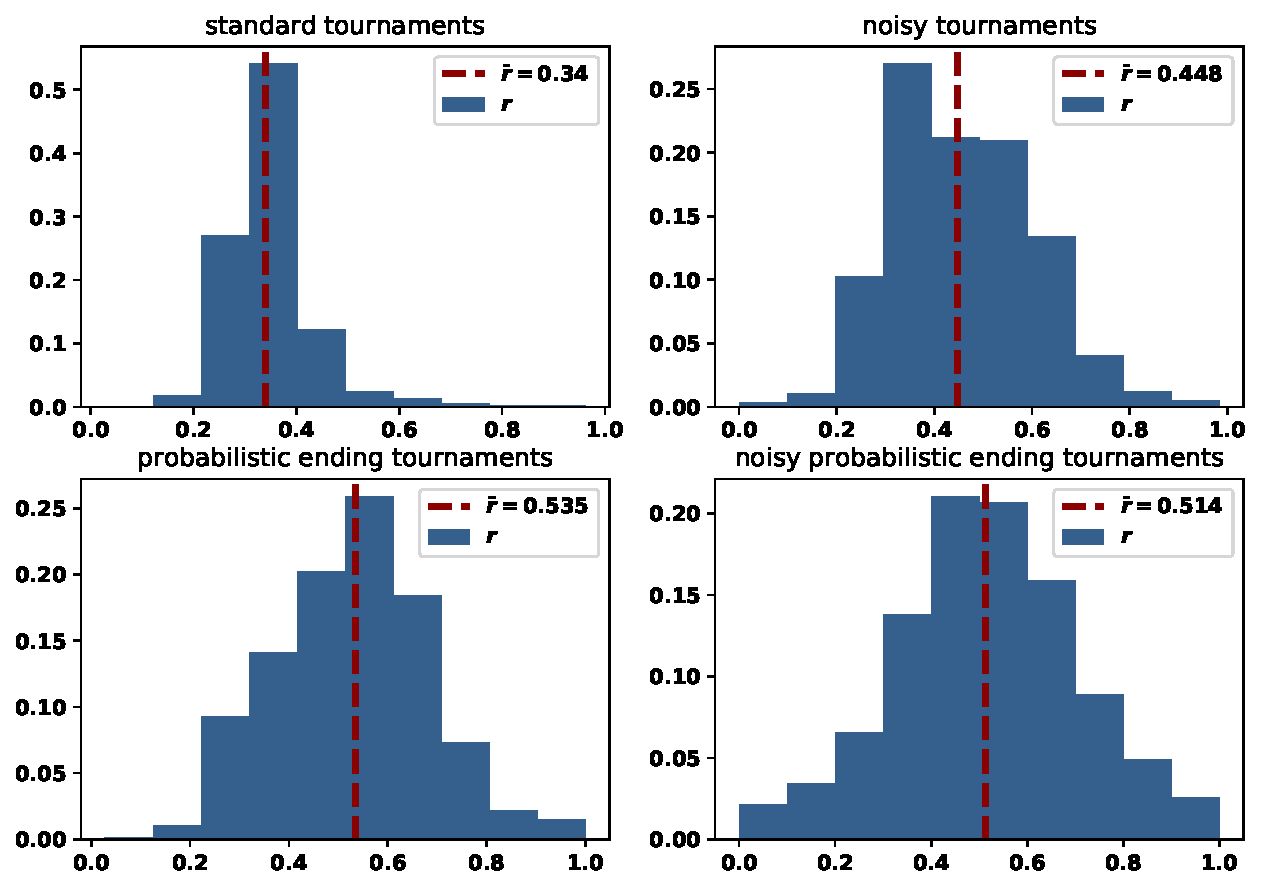
\includegraphics[width=.60\textwidth]{src/chapters/04/paper/meta-analysis-of-prisoners-dilemma-tournaments/images/tit_for_tat_r_distributions.pdf}
    \caption{Tit For Tat's $r$ distribution in tournaments. Lower values of \(r\)
    correspond to better performances. The best performance
    of the strategy has been in standard tournaments where it achieved a $\bar{r}$
    of 0.34.}
    \label{fig:tit_for_tat_r_distribution}
\end{figure}

The top 15 strategies for each tournament type based on \(\bar{r}\) are given in
Table~\ref{table:top_performances}. The data collection process was designed such
that the probabilities of noise and ending of the match varied between 0 and
1. However, commonly used values for these probabilities are values less than 0.1.
Thus,
Table~\ref{table:top_performances} also includes the top 15 strategies in noisy
tournaments with \(p_n < 0.1\) and probabilistic ending tournaments with \(p_e <
0.1\). The \(r\) distributions for the top ranked strategies of Table~\ref{table:top_performances}
are given by Figure~\ref{fig:r_distributions}.

\newcolumntype{g}{>{\columncolor{Gray}}l}
\begin{table}[!htbp]
    \begin{center}
    \resizebox{\textwidth}{!}{
        \begin{tabular}{lggllggllr}
\toprule
& \multicolumn{2}{g}{Standard} & \multicolumn{2}{c}{Noisy} & \multicolumn{2}{g}{Probabilistic ending} &  \multicolumn{2}{c}{Noisy probabilistic ending} \\
\midrule
& Name & $\bar{r}$ &                 Name & $\bar{r}$ &               Name & $\bar{r}$ &                 Name & $\bar{r}$ \\
\midrule
0  &            Evolved HMM 5 &   0.00667 &                 Grumpy &   0.14020 &          Fortress4 &   0.01266 &           Alternator &   0.30370 \\
1  &           Evolved FSM 16 &   0.00995 &                    $e$ &   0.19388 &           Defector &   0.01429 &               $\phi$ &   0.30978 \\
2  &     EvolvedLookerUp2 2 2 &   0.01064 &         Tit For 2 Tats &   0.20617 &  Better and Better &   0.01587 &                  $e$ &   0.31250 \\
3  &  Evolved FSM 16 Noise 05 &   0.01667 &  Slow Tit For Two Tats &   0.20962 &    Tricky Defector &   0.01875 &                $\pi$ &   0.31686 \\
4  &        PSO Gambler 2 2 2 &   0.02143 &           Cycle Hunter &   0.21538 &          Fortress3 &   0.02174 &    Limited Retaliate &   0.35263 \\
5  &              Evolved ANN &   0.02878 &         Risky QLearner &   0.22222 &     Gradual Killer &   0.02532 &     Anti Tit For Tat &   0.35431 \\
6  &            Evolved ANN 5 &   0.03390 &            Retaliate 3 &   0.22887 &         Aggravater &   0.02778 &          Retaliate 3 &   0.35563 \\
7  &        PSO Gambler 1 1 1 &   0.03704 &          Cycler CCCCCD &   0.23507 &             Raider &   0.03077 &  Limited Retaliate 3 &   0.35563 \\
8  &            Evolved FSM 4 &   0.04891 &            Retaliate 2 &   0.23913 &         Cycler DDC &   0.04545 &            Retaliate &   0.35714 \\
9  &         PSO Gambler Mem1 &   0.05036 &        Defector Hunter &   0.24038 &        Hard Prober &   0.05128 &          Retaliate 2 &   0.35767 \\
10 &                 Winner12 &   0.06011 &              Retaliate &   0.24177 &         SolutionB1 &   0.06024 &  Limited Retaliate 2 &   0.36134 \\
11 &             Fool Me Once &   0.06140 &    Hard Tit For 2 Tats &   0.25000 &      Meta Minority &   0.06077 &             Hopeless &   0.36842 \\
12 &                      DBS &   0.07143 &               ShortMem &   0.25286 &              Bully &   0.06081 &    Arrogant QLearner &   0.40651 \\
13 &            DoubleCrosser &   0.07200 &    Limited Retaliate 3 &   0.25316 &    Fool Me Forever &   0.07080 &    Cautious QLearner &   0.40909 \\
14 &              BackStabber &   0.07519 &      Limited Retaliate &   0.25706 &             EasyGo &   0.07101 &      Fool Me Forever &   0.41764 \\
\bottomrule
    \end{tabular}
    
    }
\end{center}
\caption{Top performances for each tournament type based on $\bar{r}$. The
results of each type are based on 11420 unique tournaments. The
results for noisy tournaments with \(p_n < 0.1\) are based on 1151 tournaments,
and for probabilistic ending tournaments with \(p_e < 0.1\) on 1139. The top
ranks indicate that trained strategies perform well in a variety of
environments, but so do simple deterministic strategies. The normalised medians
are close to 0 for most environments, except environments with noise not
restricted to 0.1 regardless of the number of turns. Noisy and noisy probabilistic
ending tournaments have the highest medians.}
\label{table:top_performances}
\end{table}

\begin{figure*}[!htbp]
    \centering
    \begin{subfigure}{0.47\textwidth}
        \centering
        \includegraphics[width=\textwidth]{src/chapters/04/paper/meta-analysis-of-prisoners-dilemma-tournaments/images/r_distribution_standard.pdf}
        \caption{$r$ distributions of top 15 strategies in standard tournaments.}\label{fig:std_results}
    \end{subfigure}
    \hfill
    \begin{subfigure}{0.47\textwidth}
        \centering
        \includegraphics[width=\textwidth]{src/chapters/04/paper/meta-analysis-of-prisoners-dilemma-tournaments/images/r_distribution_noise_subset.pdf}
        \caption{$r$ distributions of top 15 strategies in noisy tournaments with \(p_n < 0.1\).}\label{fig:noise_subset_results}
    \end{subfigure}
    \vskip\baselineskip
    \begin{subfigure}{0.485\textwidth}
        \centering
        \includegraphics[width=\textwidth]{src/chapters/04/paper/meta-analysis-of-prisoners-dilemma-tournaments/images/r_distribution_noise.pdf}
        \caption{$r$ distributions of top 15 strategies in noisy tournaments.}\label{fig:noise_results}
    \end{subfigure}
    \quad
    \begin{subfigure}{0.47\textwidth}
        \centering
        \includegraphics[width=\textwidth]{src/chapters/04/paper/meta-analysis-of-prisoners-dilemma-tournaments/images/r_distribution_probend_subset.pdf}
        \caption{\(r\) distributions of top 15 strategies in 1139 probabilistic ending
        tournaments with \(p_e < 0.1\).}
        \label{fig:probend_subset_results}
    \end{subfigure}
    \vskip\baselineskip
    \begin{subfigure}{0.485\textwidth}
        \centering
        \includegraphics[width=\textwidth]{src/chapters/04/paper/meta-analysis-of-prisoners-dilemma-tournaments/images/r_distribution_probend.pdf}
        \caption{$r$ distributions of top 15 strategies in probabilistic ending tournaments.}\label{fig:probend_results}
    \end{subfigure}
    \quad
    \begin{subfigure}{0.47\textwidth}
        \centering
        \includegraphics[width=\textwidth]{src/chapters/04/paper/meta-analysis-of-prisoners-dilemma-tournaments/images/r_distribution_probend_noise.pdf}
        \caption{$r$ distributions of top 15 strategies in noisy probabilistic ending tournaments.}
        \label{fig:probend_noise_results}
    \end{subfigure}
    \caption{\(r\) distributions of the top 15 strategies in different
    environments. A lower value of \(\bar{r}\) corresponds to a more successful
    performance. A strategy's \(r\) distribution skewed towards zero indicates
    that the strategy ranked highly in most tournaments it participated in. Most
    distributions are skewed towards zero except the distributions with
    unrestricted noise, supporting the conclusions from
    Table~\ref{table:top_performances}.}\label{fig:r_distributions}
\end{figure*}

In standard tournaments 10 out of the 15 top strategies were introduced
in~\cite{Harper2017}. These are strategies based on finite state automata (FSM),
hidden Markov models (HMM), artificial neural networks (ANN), lookup tables
(LookerUp) and stochastic lookup tables (Gambler) that have been trained using
reinforcement learning algorithms (evolutionary and particle swarm algorithms).
They have been trained to perform well against a subset of the strategies
in APL in a standard tournament, thus their performance in the
specific setting was anticipated although still noteworthy given the random
sampling of tournament participants. DoubleCrosser, BackStabber and Fool Me Once, are
strategies not from the literature but from the APL. DoubleCrosser is an extension
of BackStabber and both strategies make use of the number of turns because they are
set to defect on the last two rounds. It should be noted that these
strategies can be characterised as ``cheaters'' because the source code of the strategies
allows them to know the number of turns in a match (unless the match has a probabilistic ending). These strategies were expected to not perform as well in
tournaments where the number of turns is not specified. Finally, Winner
12~\cite{mathieu2017} and DBS~\cite{Au2006} are both from the literature.
DBS is a strategy specifically designed for noisy environments, however, it ranks
highly in standard tournaments as well. Similarly the fourth ranked player,
Evolved FSM 16 Noise 05, was
trained for noisy tournaments yet performs well in standard tournaments.
Figure~\ref{fig:std_results} shows that these strategies typically perform
well in any standard tournament in which they participate.

In the case of noisy tournaments with smaller noise \(p_n < 0.1\) the top
performing strategies
include strategies specifically designed for noisy tournaments. These are DBS,
Evolved FSM 16 Noise 05, Evolved ANN 5 Noise 05, PSO Gambler 2 2 2 Noise 05 and
Omega Tit For Tat~\cite{kendall2007iterated}. Omega Tit For Tat, another strategy designed
to break the deadlocking cycles of \(CD\) and \(DC\) that Tit For Tat can fall into in noisy
environments, places 10th. The rest of the top ranks are
occupied by strategies which performed well in standard tournaments and
deterministic strategies such as Spiteful Tit For Tat~\cite{prison}, Level
Punisher~\cite{Eckhart2015}, Eugine Nier~\cite{lesswrong}.

In contrast, the performance of the top ranked strategies in noisy environments
when \(p_n\in [0, 1]\) is bimodal. The top strategies include strategies which
decide their actions based on the cooperation to defection ratio, such as
ShortMem~\cite{Andre2013}, Grumpy~\cite{axelrodproject} and
e~\cite{axelrodproject}, and the Retaliate strategies which are designed to
defect if the opponent has tricked them more often than a given percentage of the times that
they have done the same. The bimodality of the \(r\) distributions is explained
by Figure~\ref{fig:effect_of_noise} which demonstrates that the top 6 strategies
were highly ranked due to the their performance in tournaments with \(p_n>0.5\),
and that in tournaments with \(p_n<0.5\) they
performed poorly. At a noisy level of \(0.5\) or greater, mostly cooperative strategies
become mostly defectors and vice versa.

\begin{figure}[!htbp]
    \centering
    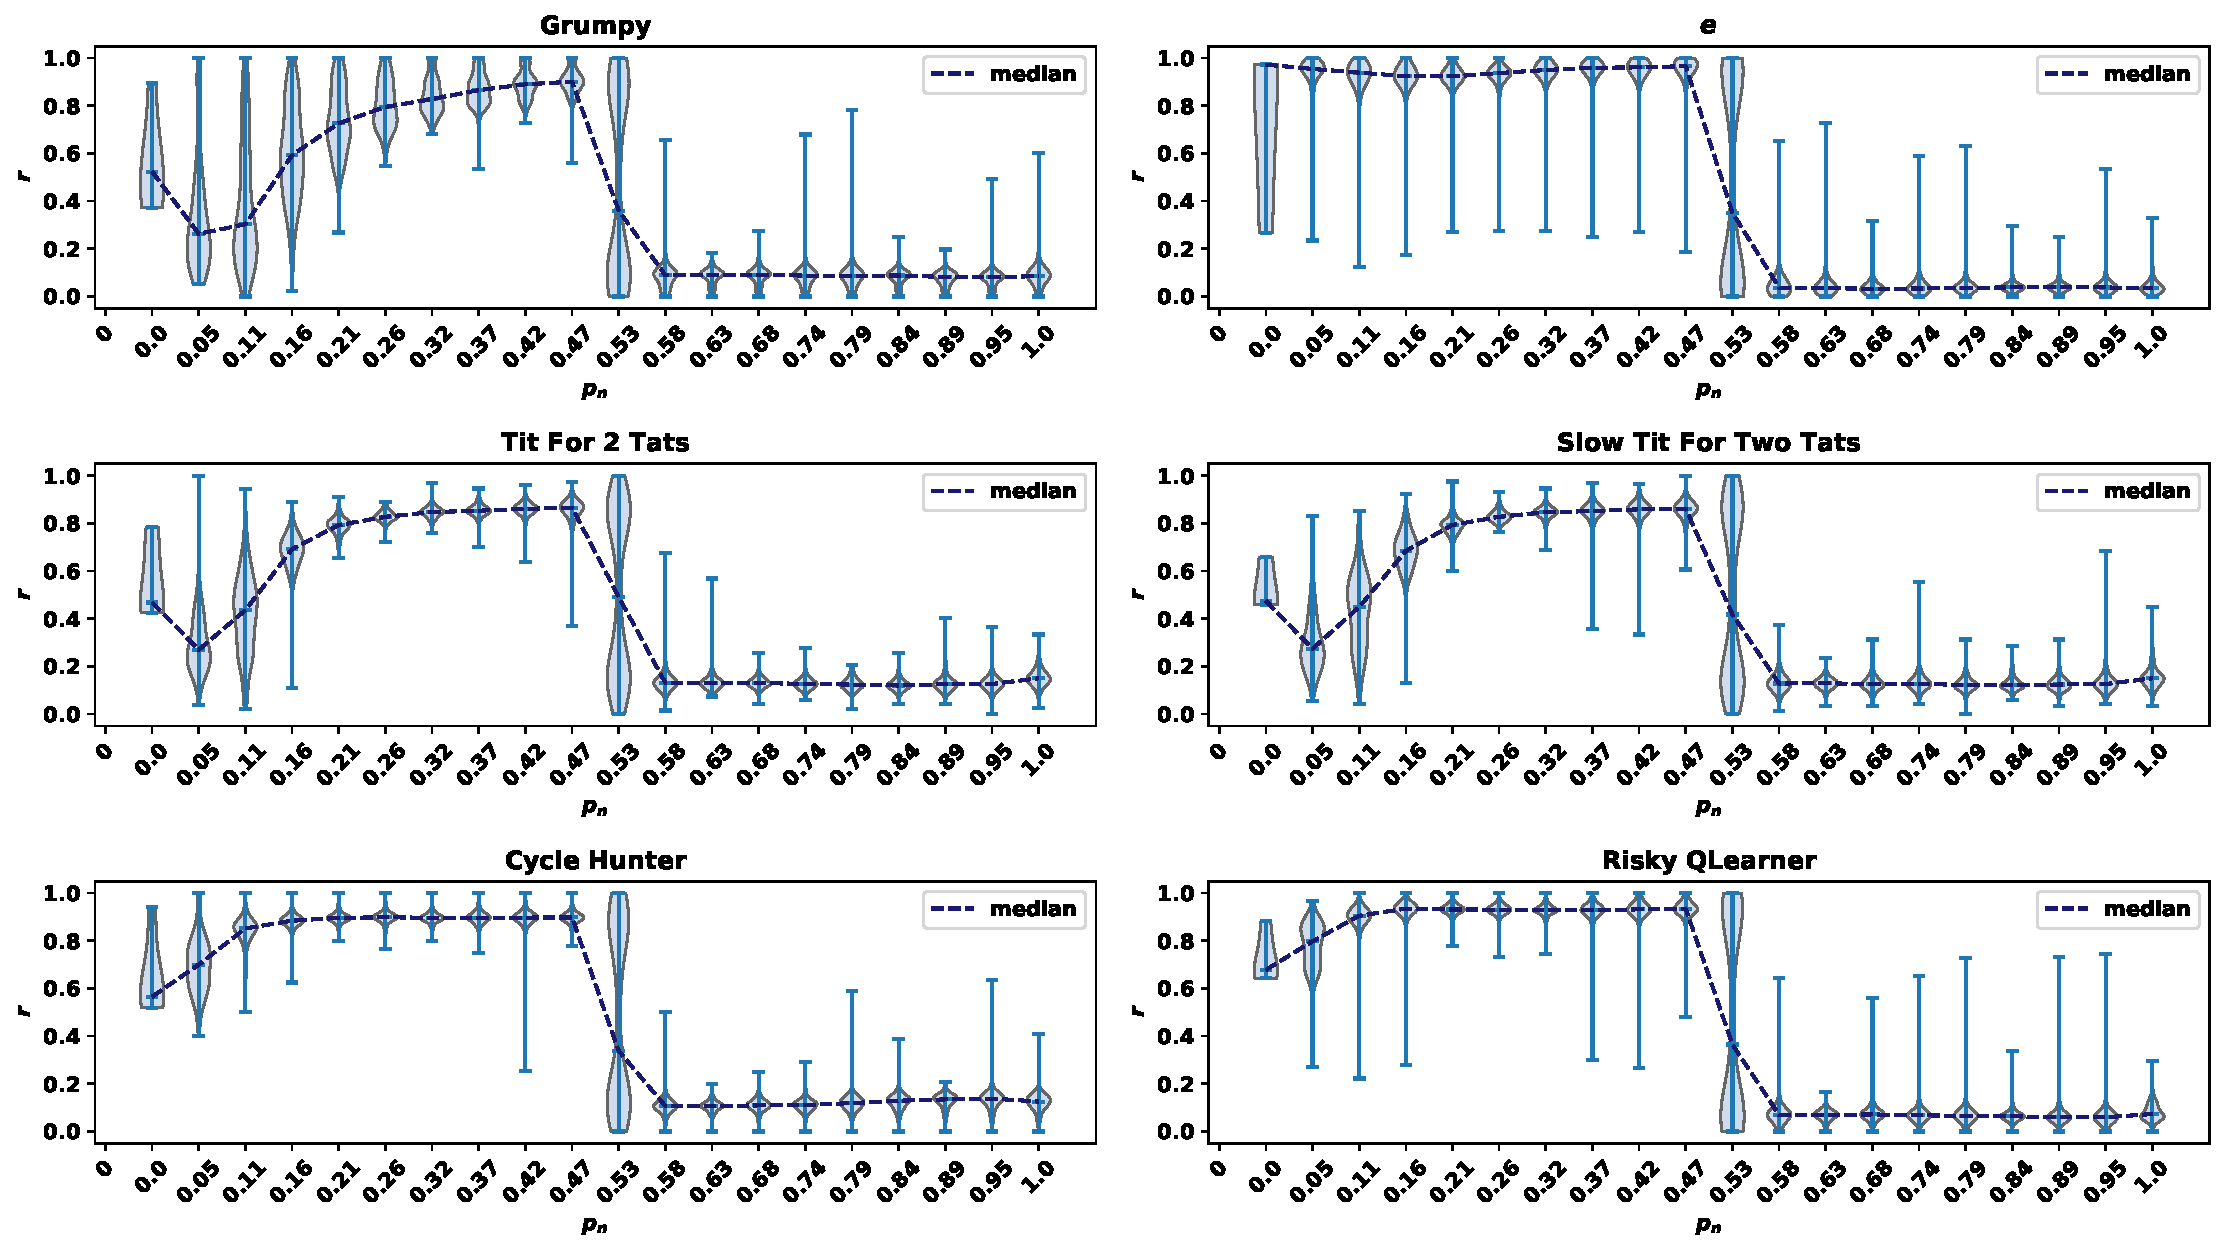
\includegraphics[width=.92\textwidth]{src/chapters/04/paper/meta-analysis-of-prisoners-dilemma-tournaments/images/noise_effect.pdf}
    \caption{Normalised rank \(r\) distributions for top 6 strategies in noisy tournaments over
    the probability of noisy ($p_n$).}
    \label{fig:effect_of_noise}
\end{figure}

The most effective strategies in probabilistic ending
tournaments with \(p_e< 0.1\) are a series of ensemble Meta strategies, trained strategies
which performed well
in standard tournaments, and Grudger~\cite{axelrodproject} and Spiteful Tit for
Tat~\cite{prison}. The Meta strategies~\cite{axelrodproject} utilise a team of
strategies and aggregate the potential actions of the team members into a single action
in various ways. Figure~\ref{fig:probend_subset_results} indicates that these strategies
performed well in any probabilistic ending tournament.

In probabilistic ending tournaments with \(p_e \in [0, 1]\) the top ranks are
mostly occupied by defecting strategies such as Better and Better, Gradual
Killer, Hard Prober (all from~\cite{axelrodproject}), Bully (Reverse Tit For
Tat)~\cite{Nachbar1992} and Defector, and a series of strategies based on finite
state automata introduced by Daniel Ashlock and Wendy Ashlock: Fortress 3,
Fortress 4 (both introduced in~\cite{Ashlock2006}), Raider~\cite{Ashlock2014}
and Solution B1~\cite{Ashlock2014}. The success of defecting strategies in
probabilistic ending tournaments is due to larger values of
\(p_e\) which lead to shorter matches (the expected number of rounds is \(1 / p_e\)), so the
impact of the PD being iterated is subdued. This is captured by the Folk
Theorem~\cite{Fudenberg2009} as defecting strategies do better when the likelihood
of the game ending in the next turn increases.
This is demonstrated by Figure~\ref{fig:effect_of_probend}, which gives the
distributions of \(r\) for the top 6 strategies in probabilistic ending tournaments
over \(p_e\).

\begin{figure}[!htbp]
    \centering
    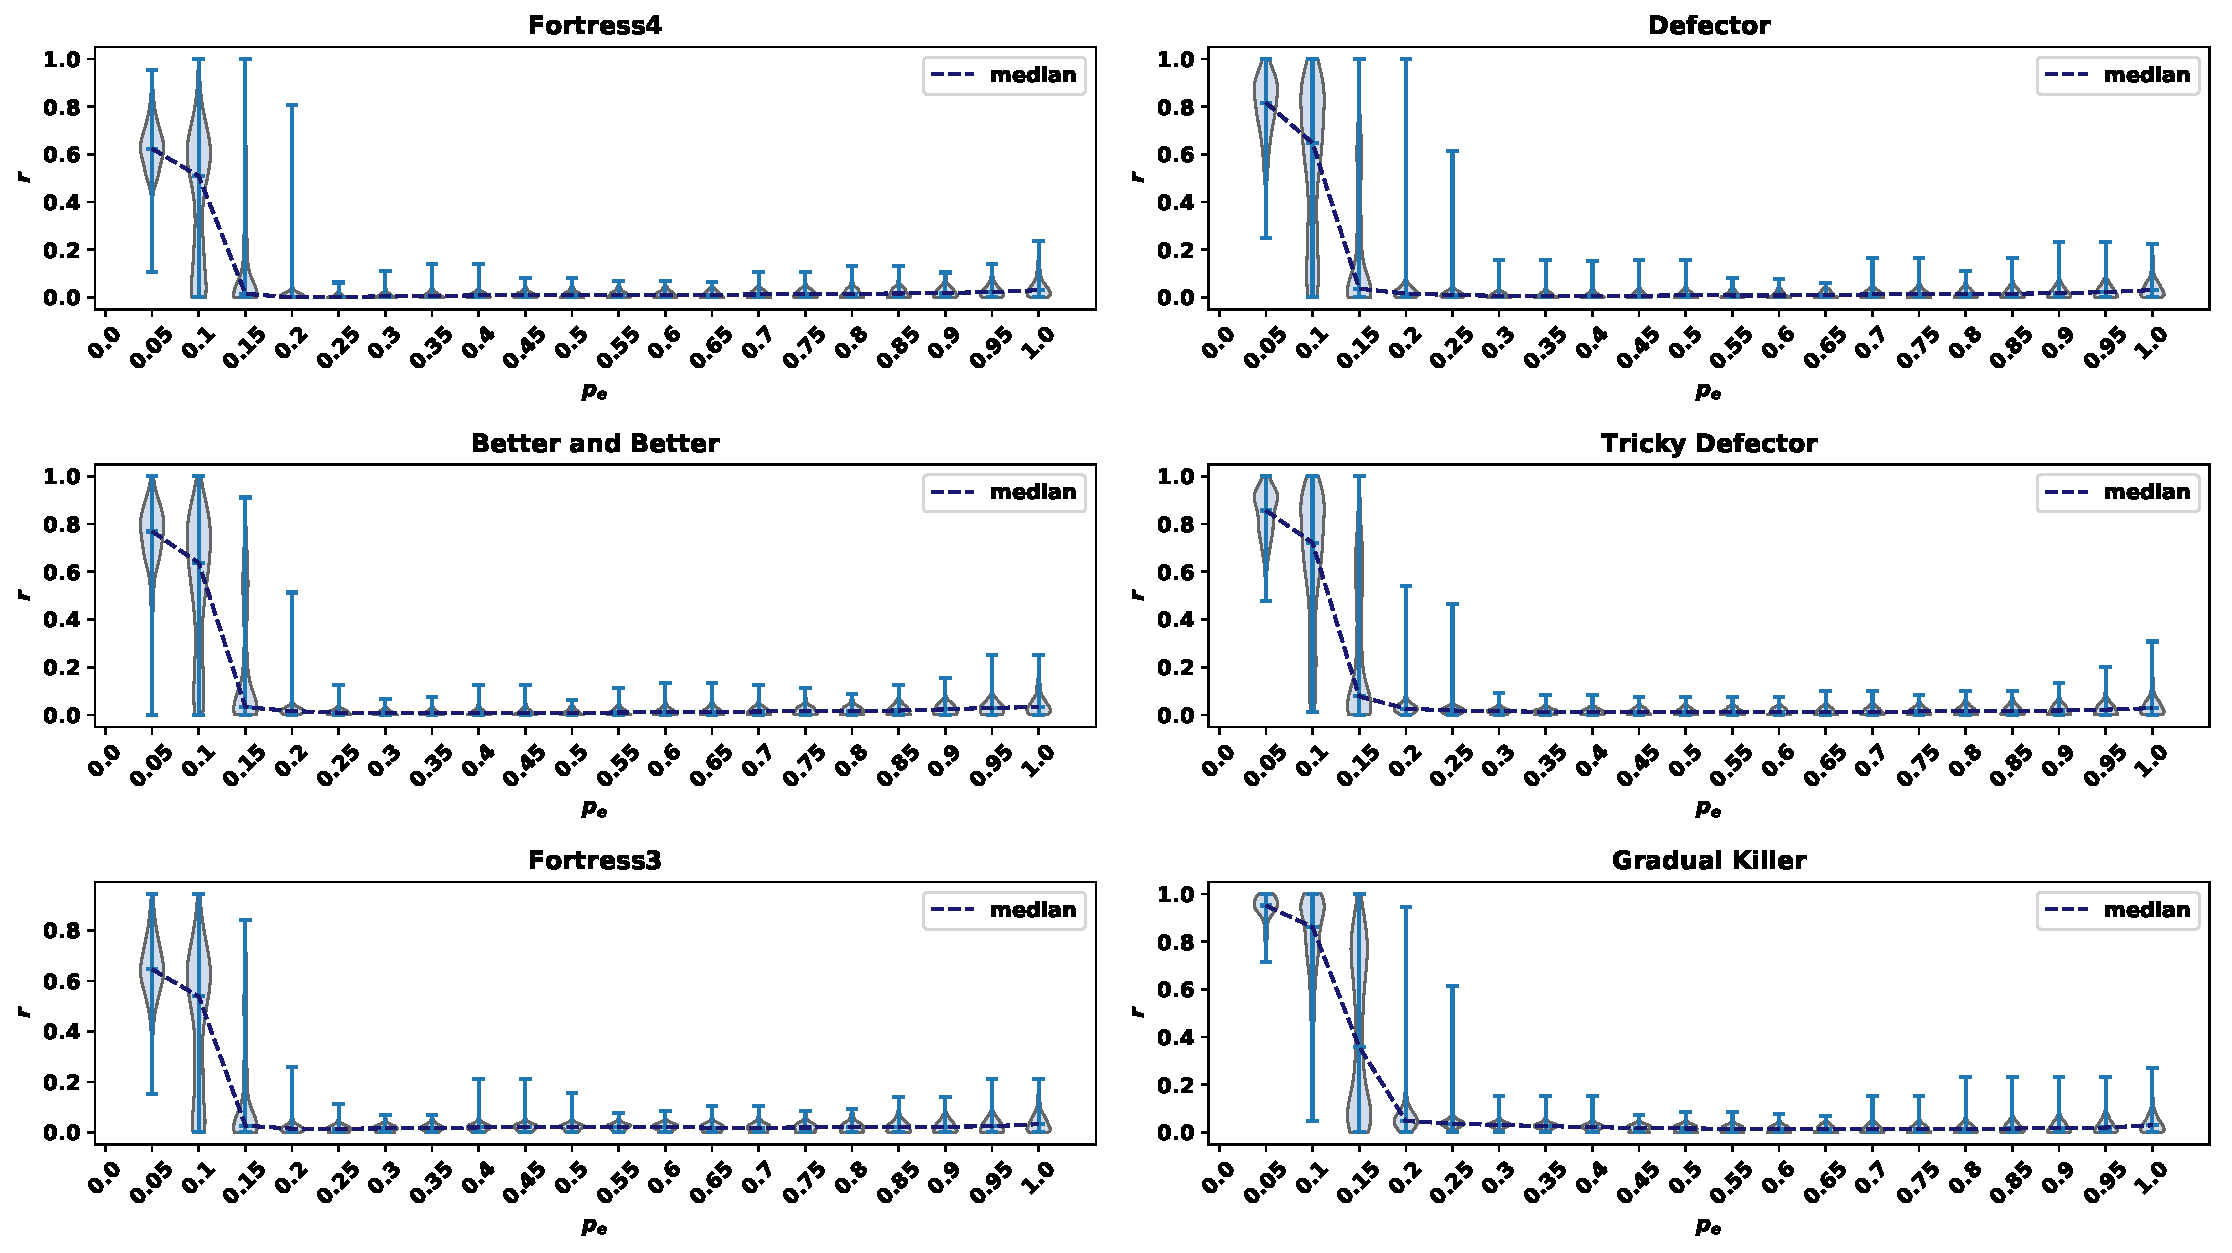
\includegraphics[width=.92\textwidth]{src/chapters/04/paper/meta-analysis-of-prisoners-dilemma-tournaments/images/folk_theorem.pdf}
    \caption{Normalised rank \(r\) distributions for top 6 strategies in probabilistic ending tournaments
    over $p_e$. The 6 strategies start of with a high median rank,
    however, their ranked decreased as the the probability of the game ending
    increased and at the point of \(p_e = 0.1\).}
    \label{fig:effect_of_probend}
\end{figure}

The top performances in tournaments with both noise and a probabilistic ending
and the top performances over the entire data set have the largest median values
compared to the top rank strategies of the other tournament types,
Figure~\ref{fig:probend_noise_results} and Figure~\ref{fig:overall_results}. The
\(\bar{r}\) for the top strategy is approximately at 0.3, indicating that the
most successful strategy can on average just place in the top 30\% of the
competition.

\begin{table}[!htbp]
    \centering
    \resizebox{.3\textwidth}{!}{
    \begin{tabular}{lr}
\toprule
Name                       &     \(\bar{r}\) \\
\midrule
Limited Retaliate 3        &            0.286 \\
Retaliate 3                &            0.297 \\
Retaliate 2                &            0.302 \\
Limited Retaliate 2        &            0.304 \\
Limited Retaliate          &            0.311 \\
Retaliate                  &            0.317 \\
BackStabber                &            0.324 \\
DoubleCrosser              &            0.331 \\
Nice Meta Winner           &            0.350 \\
PSO Gambler 2 2 2 Noise 05 &            0.351 \\
Grudger                    &            0.352 \\
NMWE Memory One            &            0.357 \\
Evolved HMM 5              &            0.358 \\
Nice Meta Winner Ensemble  &            0.359 \\
Forgetful Fool Me Once     &            0.359 \\
\bottomrule
\end{tabular}
}
    \caption{Top performances over all the tournaments. The top ranks include
    strategies that have been previously mentioned. The set of Retaliate
    strategies occupy the top spots followed by BackStabber and DoubleCrosser.
    The distributions of the Retaliate strategies have no statistical
    difference. PSO Gambler and Evolved HMM 5 are trained strategies introduced
    in~\cite{Harper2017} and Nice Meta Winner and NMWE Memory One are strategies
    based on teams. Grudger is a strategy from Axelrod's original tournament and
    Forgetful Fool Me Once is based on the same approach as
    Grudger.}\label{table:overall_results}
\end{table}

\begin{figure}[!htbp]
        \centering
        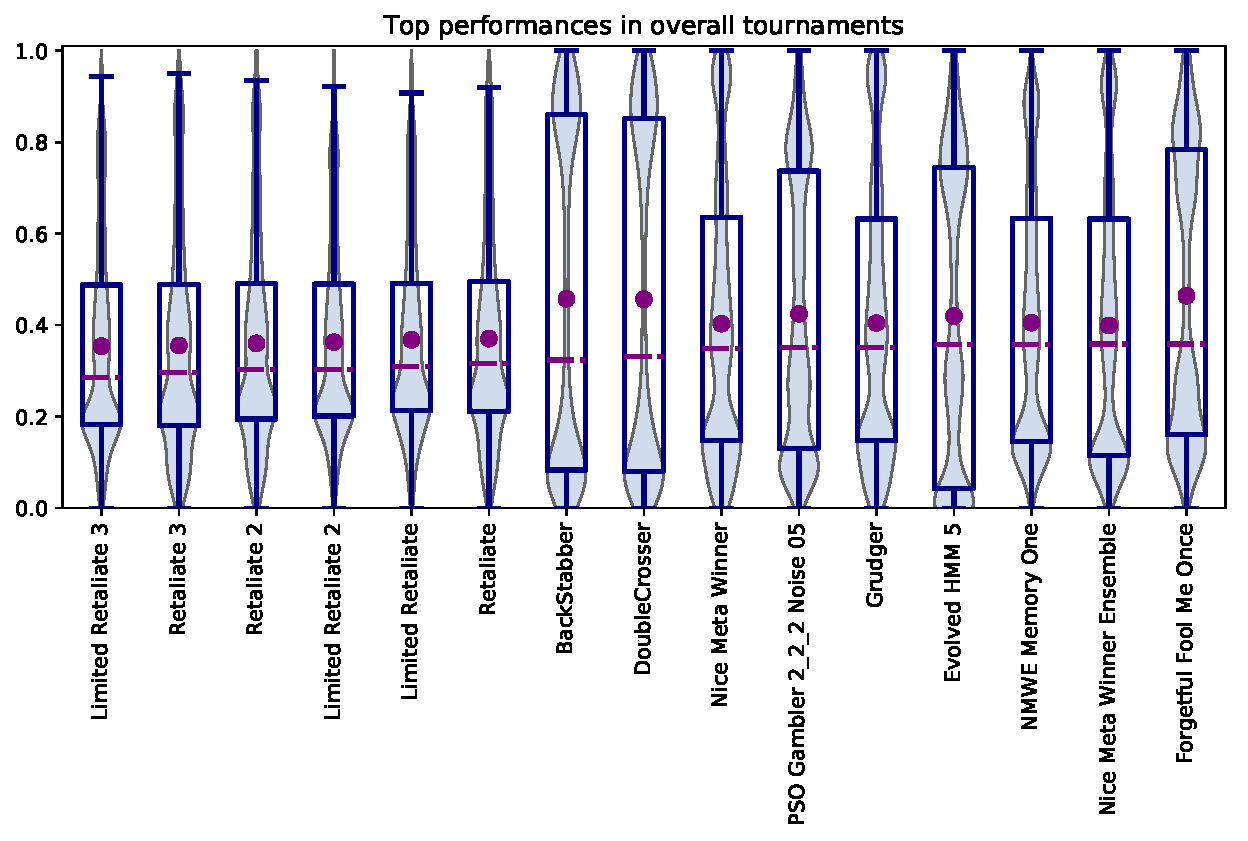
\includegraphics[width=.65\textwidth]{src/chapters/04/paper/meta-analysis-of-prisoners-dilemma-tournaments/images/performance_merged.pdf}
        \caption{\(r\) distributions for best performed strategies in the data set~\cite{Glynatsi2019_meta}.
        A lower value of \(\bar{r}\) corresponds to a more successful
        performance.}
        \label{fig:overall_results}
\end{figure}

On the whole, the analysis of this section has shown that:

\begin{itemize}
    \item In standard tournaments the dominating strategies were
    strategies that had been trained using reinforcement learning techniques.
    \item In noisy environments where the noise probability strictly less than
    0.1 was considered, the successful strategies were strategies specifically
    designed or trained for noisy environments.
    \item In probabilistic ending tournaments most of the highly ranked
    strategies were defecting strategies and trained finite state automata, all
    by the authors of~\cite{Ashlock2006, Ashlock2014}. These strategies ranked
    high due to their performance in tournaments where the probability of the
    game ending after each turn was bigger than 0.1.
    \item In probabilistic tournaments with \(p_e\) less than 0.1 the highly
    ranked strategies were strategies based on the behaviour of others.
    \item From the collection of strategies considered here,  no strategy can be
    consistently successful in noisy environments, except if the value of noise
    is constrained to less than a 0.1.
\end{itemize}

Though there is not a single strategy that repeatably outranks all others in any
of the distinct tournament types, or even across the tournament types, there
are specific types of strategies have been repeatably ranked in the top ranks.
These have been strategies that have been trained, strategies that retaliate,
and strategies that would adapt their behaviour based on preassigned rules
to achieve the highest outcome. These results contradict some of Axelrod's suggestions,
and more specifically, the suggestions `Do not be clever' and `Do not be envious'.
The features and properties contributing a strategy's success are further
explored in section~\ref{section:evaluation_of_performance}.

\section{Evaluation of performance}\label{section:evaluation_of_performance}

This section examines the performance of the strategies based on features of strategies described in
Table~\ref{table:manual_features}. These features are measures regarding a
strategy's behaviour from the tournaments the strategies competed in as well as
intrinsic properties such as whether a strategy is deterministic or stochastic.

\newcolumntype{g}{>{\columncolor{Gray}}c}
\begin{table}[!htbp]
    \begin{center}
    \resizebox{.99\textwidth}{!}{
    \begin{tabular}{gcgcgc}
    \toprule
    feature & feature explanation &  source & value type & min value & max value \\
    \midrule
stochastic  &  If a strategy is stochastic & strategy classifier from APL & boolean  & Na &  Na \\
makes use of game &  If a strategy makes used of the game information & strategy classifier from APL & boolean  & Na &  Na \\
makes use of length &  If a strategy makes used of the number of turns & strategy classifier from APL & boolean  & Na &  Na \\
memory usage &  The memory size of a strategy divided by the number of turns & memory size from APL & float & 0 &  1 \\
SSE & A measure of how far a strategy is from ZD behaviour & method described in~\cite{Knight2019} & float & 0 & 1 \\
max cooperating rate $(C_{\text{max}})$  & The biggest cooperating rate in a given tournament  & result summary  & float & 0 & 1\\
min cooperating rate $(C_{\text{min}})$ & The smallest cooperating rate in a given tournament  & result summary  & float & 0 & 1\\
median cooperating rate $(C_{\text{median}})$ & The median cooperating rate in a given tournament  & result summary  & float & 0 & 1\\
mean cooperating rate $(C_{\text{mean}})$ & The mean cooperating rate in a given tournament  & result summary  & float & 0 & 1 \\
$C_r$ / $C_{\text{max}}$ & A strategy's cooperating rate divided by the maximum & result summary  & float & 0 & 1 \\
$C_{\text{min}}$ / $C_r$ & A strategy's cooperating rate divided by the minimum & result summary  & float & 0 & 1 \\
$C_r$ / $C_{\text{median}}$ & A strategy's cooperating rate divided by the median  & result summary  & float & 0 & 1\\
$C_r$ / $C_{\text{mean}}$ & A strategy's cooperating rate divided by the mean & result summary  & float & 0 & 1 \\
$C_r$ & The cooperating ratio of a strategy & result summary  & float & 0 & 1 \\
$CC$ to $C$ rate & The probability a strategy will cooperate after a mutual cooperation & result summary  & float & 0 & 1\\
$CD$ to $C$ rate & The probability a strategy will cooperate after being betrayed by the opponent & result summary  & float & 0 & 1 \\
$DC$ to $C$ rate & The probability a strategy will cooperate after betraying the opponent & result summary  & float & 0 & 1 \\
$DD$ to $C$ rate & The probability a strategy will cooperate after a mutual defection & result summary  & float & 0 & 1 \\
$p_n$ & The probability of a player's action being flip at each interaction & trial summary & float & 0 & 1 \\
$n$ & The number of turns & trial summary & integer & 1 & 200 \\
$p_e$ & The probability of a match ending in the next turn & trial summary & float & 0 & 1 \\
$N$ & The number of strategies in the tournament & trial summary & integer & 3 & 195 \\
$k$ & The number of repetitions of a given tournament & trial summary & integer & 10 & 100 \\
    \bottomrule
        \end{tabular}}
    \end{center}
    \caption{The features which are included in the performance evaluation
    analysis. Stochastic, makes use of length and makes use of game are APL
    classifiers that determine whether a strategy is stochastic or deterministic,
    whether it makes use of the number of turns or the game's payoffs. The
    memory usage is calculated as the number of turns the strategy considers to
    make an action (which is specified in the APL) divided by the number of
    turns. The SSE (introduced in~\cite{Knight2019}) shows how close a strategy
    is to behaving as a ZDs, and subsequently, in an extortionate way. The
    method identifies the ZDs closest to a given strategy and calculates the
    algebraic distance between them, defined as SSE. More details on the measure
    are presented in Chapter~\ref{chapter:memory_one}. A SSE value of 1 indicates
    no extortionate behaviour at all whereas a value of 0 indicates that a
    strategy is behaving as a ZDs. The rest of the features considered are the $CC$
    to $C$, $CD$ to $C$, $DC$ to $C$, and $DD$ to $C$ rates as well as
    cooperating ratio of a strategy, the minimum (\(C_{min}\)), maximum
    (\(C_{max}\)), mean (\(C_{mean}\)) and median (\(C_{median}\)) cooperating
    ratios of each tournament.}
    \label{table:manual_features}
\end{table}

The memory usage of strategies is the number of
rounds of play used by the strategy divided by the number of turns in each match.
For example, Winner12 uses the previous two rounds of play, and if participating
in a match with 100 turns its memory usage would be 2/100.
For strategies with an infinite memory size, for example Evolved
FSM 16 Noise 05, memory usage is equal to 1.
Note that for tournaments with a probabilistic
ending the number of turns was not collected, so the memory usage feature is not
used for probabilistic ending tournaments.

The correlation coefficients between the features of
Table~\ref{table:manual_features} the median score and the median normalised
rank are given by Table~\ref{table:correlations}. The correlation coefficients
between all features of Table~\ref{table:manual_features} have been calculated
and a graphical representation can be found in the
Appendix~\ref{app:correlations}.

\newcolumntype{g}{>{\columncolor{Gray}}c}
\begin{table}[!htbp]
    \begin{center}
    \resizebox{.9\textwidth}{!}{
        \begin{tabular}{lggccggccggg}
    \toprule
    &  \multicolumn{2}{g}{Standard} & \multicolumn{2}{c}{Noisy} & \multicolumn{2}{g}{Probabilistic ending} &  \multicolumn{2}{c}{Noisy probabilistic ending} &  \multicolumn{2}{g}{Overall} \\
\midrule
{} &  $r$ &  median score &  $r$ &  median score &  $r$ &  median score &  $r$ &  median score &  $r$ &  median score\\
\midrule
$CC$ to $C$ rate     & -0.501 &  0.501 &   0.414 &  -0.504 &   0.408 &  -0.323 &   0.260 &   0.022 &  -0.501 &  0.501 \\
$CD$ to $C$ rate     &  0.226 & -0.199 &   0.456 &  -0.330 &   0.320 &  -0.017 &   0.205 &  -0.220 &   0.226 & -0.199 \\
$C_r$                & -0.323 &  0.384 &   0.711 &  -0.678 &   0.714 &  -0.832 &   0.579 &  -0.135 &  -0.323 &  0.384 \\
$C_r$ / $C_{max}$    & -0.323 &  0.381 &   0.616 &  -0.551 &   0.714 &  -0.833 &   0.536 &  -0.116 &  -0.323 &  0.381 \\
$C_r$ / $C_{mean}$   & -0.331 &  0.358 &   0.731 &  -0.740 &   0.721 &  -0.861 &   0.649 &  -0.621 &  -0.331 &  0.358 \\
$C_r$ / $C_{median}$ & -0.331 &  0.353 &   0.652 &  -0.669 &   0.712 &  -0.852 &   0.330 &  -0.466 &  -0.331 &  0.353 \\
$C_r$ / $C_{min}$    &  0.109 & -0.080 &  -0.358 &   0.250 &  -0.134 &   0.150 &  -0.368 &   0.113 &   0.109 & -0.080 \\
$C_{max}$            & -0.000 &  0.049 &   0.000 &   0.023 &  -0.000 &   0.046 &   0.000 &  -0.004 &  -0.000 &  0.049 \\
$C_{mean}$           & -0.000 &  0.229 &  -0.000 &   0.271 &   0.000 &   0.200 &   0.000 &   0.690 &  -0.000 &  0.229 \\
$C_{median}$         &  0.000 &  0.209 &  -0.000 &   0.240 &  -0.000 &   0.187 &  -0.000 &   0.673 &   0.000 &  0.209 \\
$C_{min}$            &  0.000 &  0.084 &   0.000 &  -0.017 &  -0.000 &   0.007 &  -0.000 &   0.041 &   0.000 &  0.084 \\
$DC$ to $C$ rate     &  0.127 & -0.100 &   0.509 &  -0.504 &  -0.018 &   0.033 &   0.341 &  -0.016 &   0.127 & -0.100 \\
$DD$ to $C$ rate     &  0.412 & -0.396 &   0.533 &  -0.436 &  -0.103 &   0.176 &   0.378 &  -0.263 &   0.412 & -0.396 \\
$N$                  &  0.000 & -0.009 &  -0.000 &   0.002 &  -0.000 &   0.003 &  -0.000 &   0.001 &   0.000 & -0.009 \\
$k$                  &  0.000 & -0.002 &  -0.000 &   0.003 &  -0.000 &   0.001 &  -0.000 &  -0.008 &   0.000 & -0.002 \\
$n$                  &  0.000 & -0.125 &  -0.000 &  -0.024 &       - &       - &       - &       - &   0.000 & -0.125 \\
$p_e$                &      - &      - &        - &     - &    0.000 &   0.165 &   0.000 &  -0.058 &  -0.001 &  0.001 \\
$p_n$                &      - &      - &  -0.000 &   0.207 &       - &       - &  -0.000 &  -0.650 &   0.002 & -0.000 \\
Make use of game     & -0.003 & -0.022 &   0.025 &  -0.082 &  -0.053 &  -0.108 &   0.013 &  -0.016 &  -0.003 & -0.022 \\
Make use of length   & -0.158 &  0.124 &   0.005 &  -0.123 &  -0.025 &  -0.090 &   0.014 &  -0.016 &  -0.154 &  0.117 \\
SSE                  &  0.473 & -0.452 &   0.463 &  -0.337 &  -0.156 &   0.223 &   0.305 &  -0.259 &   0.473 & -0.452 \\
memory usage         & -0.082 &  0.095 &  -0.007 &  -0.017 &       - &     - &     - &           - &  -0.084 &  0.095 \\
stochastic           &  0.006 & -0.024 &   0.022 &  -0.026 &   0.002 &  -0.130 &   0.021 &  -0.013 &   0.006 & -0.024 \\
\bottomrule
\end{tabular}

    }
\end{center}
\caption{Correlations between the features of Table~\ref{table:manual_features}
and the normalised rank and the median score.}\label{table:correlations}
\end{table}

In standard tournaments the features $CC$ to $C$, $C_r$, $C_r / C_{\text{max}}$
and the cooperating ratio compared to $C_{\text{median}}$ and $C_{\text{mean}}$
have a moderately negative effect on the normalised rank (smaller rank is better), and a moderate positive
on the median score. The SSE error and the $DD$ to $C$ rate have the opposite
effects. Thus, in standard tournaments behaving cooperatively corresponds to a
more successful performance. Even though being nice generally pays off
that does not hold against defective strategies. Being more cooperative after a mutual
defection, that is not retaliating, is associated to lesser overall success in terms of normalised rank.
Figure~\ref{fig:rates_of_winners_in_standard_tournaments} confirms that the
winners of standard tournaments always cooperate after a mutual cooperation and
almost always defect after a mutual defection.

\begin{figure}[!htbp]
    \centering
    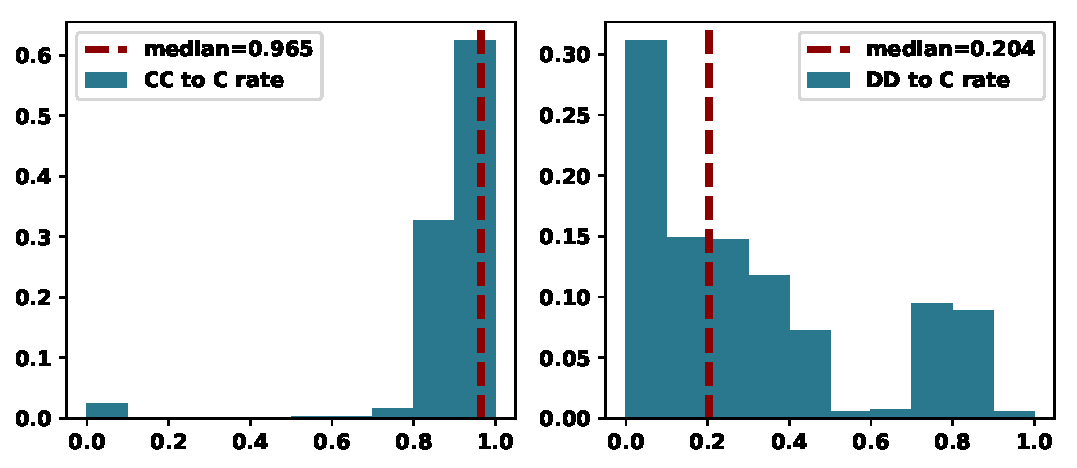
\includegraphics[width=.8\textwidth]{src/chapters/04/paper/meta-analysis-of-prisoners-dilemma-tournaments/images/rates_of_winners_in_standard_tournaments.pdf}
    \caption{Distributions of $CC$ to $C$ and $DD$ to $C$ for the winners in
    standard tournaments.}\label{fig:rates_of_winners_in_standard_tournaments}
\end{figure}

Compared to standard tournaments, in both noisy and in probabilistic ending
tournaments the higher the rates of cooperation the lower a strategy's success
and median score. A strategy would want to cooperate less than both
the mean and median cooperator in such settings. In probabilistic ending
tournaments the correlation coefficients have larger values, indicating a
stronger effect. Thus a strategy will be punished more by its cooperative
behaviour in probabilistic ending environments, supporting the results of
section~\ref{section:evaluation_of_performance}
as well. The distributions of the $C_r$ of the winners in
both tournaments are given by Figure~\ref{fig:c_r_distributions}. It confirms
that the winners in noisy tournaments cooperated less than 35\% of the time
and in probabilistic ending tournaments less than 10\%.
In noisy probabilistic ending tournaments and over all the tournaments' results,
the only features that had a moderate effect are $C_r/C_{\text{mean}},
C_r/C_{\text{max}}$ and $C_r$. In such environments cooperative behaviour
appears to be punished less than in noisy and probabilistic ending
tournaments.

\begin{figure}[!htbp]
    \centering
    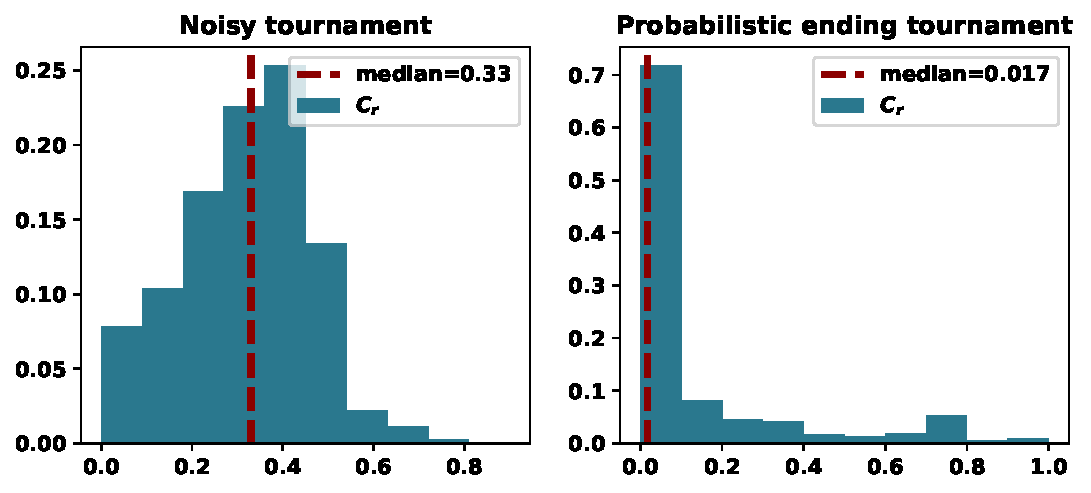
\includegraphics[width=.8\textwidth]{src/chapters/04/paper/meta-analysis-of-prisoners-dilemma-tournaments/images/c_r_winners_tournaments.pdf}
    \caption{$C_r$ distributions of the winners in noisy and in probabilistic
    ending tournaments.}\label{fig:c_r_distributions}
\end{figure}

A multivariate linear regression has been fitted to model the relationship between
the features and the normalised rank. Based on the graphical representation of
the correlation matrices given in Appendix~\ref{app:correlations} several of the
features are highly correlated and have been removed
before fitting the linear regression model. The features included are given
by Table~\ref{table:linear_regression} alongside their corresponding \(p\) values
in the distinct tournaments and their regression coefficients.

\newcolumntype{g}{>{\columncolor{Gray}}c}
\begin{table}[h]
    \begin{center}
\resizebox{\textwidth}{!}{
    \input{src/chapters/04/paper/meta-analysis-of-prisoners-dilemma-tournaments/paper/regression_table.tex}}
    \end{center}
    \caption{Results of multivariate linear regressions with \(r\) as the dependent variable.
    \(R\) squared is reported for each model.}
    \label{table:linear_regression}
\end{table}

A multivariate linear regression has also be fitted on the median score. The
coefficients and \(p\) values of the features can be found in
Appendix~\ref{app:further_regression}. The results of the two methods
are in agreement.

The feature \(C_{r} / C_{\text{mean}}\) has a statistically significant effect
across all models and a high regression coefficient. It has both a positive and
negative impact on the normalised rank depending on the environment. For
standard tournaments, Figure~\ref{fig:discussion_standard} gives the
distributions of several features for the winners of standard tournaments. The
\(C_{r} / C_{\text{mean}}\) distribution of the winner is also given in
Figure~\ref{fig:discussion_standard}. A value of \(C_r / C_{\text{mean}} = 1\)
implies that the cooperating ratio of the winner was the same as the mean
cooperating ratio of the tournament, and in standard tournaments, the median is
1. Therefore, an effective strategy in standard tournaments was the mean
cooperator of its respective tournament.

The distributions of SSE and \(CD\) to \(C\) rate for the winners of standard
tournaments are also given in Figure~\ref{fig:discussion_standard}. The SSE
distributions for the winners indicate that the strategy behaved in a ZD way in
several tournaments, however, not constantly. The winners participated in
matches where they did not try to extortionate their opponents. Furthermore, the
\(CD\) to \(C\) distribution indicates that if a strategy were to defect against
the winners the winners would reciprocate on average with a probability of 0.5.

\begin{figure}[!htbp]
    \centering
        \centering
        \includegraphics[width=\textwidth]{src/chapters/04/paper/meta-analysis-of-prisoners-dilemma-tournaments/images/standard_discussion.pdf}
        \caption{Distributions of \(C_r / C_{\text{mean}}\), SSE and \(CD\) to \(C\) ratio
        for the winners of standard tournaments. A
        value of \(C_r / C_{\text{mean}} = 1\) imply that the cooperating ratio of the
        winner was the same as the mean cooperating ratio of the tournament. An SSE distribution
        skewed towards 0 indicates a extortionate behaviour by the strategy.}
        \label{fig:discussion_standard}
\end{figure}

Similarly for the rest of the different tournaments types, and the entire data
set the distributions of \(C_r / C_{\text{mean}}\), SSE and \(CD\) to \(C\) ratio
are given by Figures~\ref{fig:discussion_noisy},~\ref{fig:discussion_probend},
\ref{fig:discussion_probend_noisy} and~\ref{fig:discussion_entire_data}.

Based on the \(C_r / C_{\text{mean}}\) distributions the successful strategies
have adapted differently to the mean cooperator depending on the tournament
type. In noisy tournaments where the median of the distribution is at 0.67, and
thereupon the winners cooperated 67\% of the time the mean cooperator did. In
tournaments with noise and a probabilistic ending the winners cooperated 60\%,
whereas in settings that the type of the tournament can vary between all the
types the winners cooperated 67\% of the time the mean cooperator did. Lastly,
in probabilistic ending tournaments above more defecting
strategies prevail (section~\ref{section:top_performances}), and this result is
reflected here.

\begin{figure}[!htbp]
    \centering
        \centering
        \includegraphics[width=\textwidth]{src/chapters/04/paper/meta-analysis-of-prisoners-dilemma-tournaments/images/noisy_discussion.pdf}
        \caption{Distributions of \(C_r / C_{\text{mean}}\), SSE and \(CD\) to \(C\) ratio
        for the winners of noisy tournaments.}
        \label{fig:discussion_noisy}
\end{figure}

The probability of noise has been observed to substantially affect optimal
behaviour.
Figure~\ref{fig:compared_to_mean_over_noise_probability} gives the ratio \(C_r /
C_{\text{mean}}\) for the winners in tournaments with noise, over the
probability of noise. From Figure~\ref{fig:noisy_discussion_over_noise} it is
clear that the cooperating only 67\% of the time the mean cooperator did is
optimal only when \(p_n \in [0.2, 0.4)\) and \(p_n \in [0.6, 0.7]\). In
environments with \(p_n < 0.1\) the winners want to be close to the mean
cooperator, similarly to standard tournaments, and as the probability of noise
is exceeding 0.5 (where the game is effectively inverted) strategies should
aim to be less and less cooperative.

Figure~\ref{fig:compared_to_mean_over_noise_probability} gives \(C_r /
C_{\text{mean}}\) for the winners over \(p_n\) in tournaments with noise and a
probabilistic ending. The optimal proportions of cooperations are different
now that the number of turns is not fixed, successful strategies
want to be more defecting that the mean cooperator, that only changes when
\(p_n\) approaches 0.5. Figure~\ref{fig:compared_to_mean_over_noise_probability}
demonstrates how the adjustments to \(C_r /C_{\text{mean}}\) change over the
noise in the to the environment, and thus supports how important adapting to
the environment is for a strategy to be successful.

\begin{figure}[!htbp]
    \centering
    \begin{subfigure}{0.485\textwidth}
        \centering
        \includegraphics[width=\textwidth]{src/chapters/04/paper/meta-analysis-of-prisoners-dilemma-tournaments/images/noisy_discussion_over_noise.pdf}
        \caption{\(C_r / C_{\text{mean}}\) distribution for winners in noisy tournaments over
        \(p_n\).}\label{fig:noisy_discussion_over_noise}
    \end{subfigure}
    \hfill
    \begin{subfigure}{0.485\textwidth}
        \centering
        \includegraphics[width=\textwidth]{src/chapters/04/paper/meta-analysis-of-prisoners-dilemma-tournaments/images/noisy_probend_discussion_over_noise.pdf}
        \caption{\(C_r / C_{\text{mean}}\) distribution for winners in noisy probabilistic ending tournaments over
        \(p_n\).}\label{fig:noisy_probend_discussion_over_noise}
    \end{subfigure}
    \caption{\(C_r / C_{\text{mean}}\) distributions over intervals of \(p_n\).
    These distributions model the optimal proportion of cooperation
    compared to \(C_{\text{mean}}\) as a function of (\(p_n\)).}
    \label{fig:compared_to_mean_over_noise_probability}
\end{figure}

The distributions of the SSE across the tournament types suggest that successful
strategies exhibit some extortionate behaviour, but not constantly.
ZDs are a set of strategies that are often envious as they try to exploit their
opponents. The winners of the tournaments considered in this work are
envious, but not as much as many ZDs.
Though the exact interactions between the matches have not been recorded here,
the work of~\cite{Harper2017} which introduced the trained strategies that
appeared in the top ranked strategies of section~\ref{section:top_performances}
did. In~\cite{Harper2017} it was shown that clever strategies managed to achieve
mutual cooperation with stronger strategies whilst exploiting the weaker
strategies. This could explain the clever winners
of this analysis, and would explain the SSE distributions. This could also
be the reason why ZDs fail to appear in the tops ranks -- they try to exploit
all opponents and cannot actively adapt back to mutual cooperation against
stronger strategies, which requires more depth of memory. Note that
ZDs also tend to perform poorly in population games for a similar reason: they
attempt to exploit other players using ZDs, failing to form a cooperative
sub population~\cite{Knight2018}. This makes them good invaders but poor resisters of invasion.

\begin{figure}[!htbp]
    \centering
        \centering
        \includegraphics[width=\textwidth]{src/chapters/04/paper/meta-analysis-of-prisoners-dilemma-tournaments/images/probend_discussion.pdf}
        \caption{Distributions of \(C_r / C_{\text{mean}}\), SSE and \(CD\) to \(C\) ratio
        for the winners of probabilistic ending tournaments.}
        \label{fig:discussion_probend}
\end{figure}

The distributions of the \(CD\) to \(C\) rate evaluate the behaviour of a
successful strategy after its opponent has defected against it. In standard
tournaments it was observed that a successful strategy reciprocates with a
probability of 0.5, and in a setting that the type
of the tournament can vary between all the examined types a winning strategy
would reciprocate on average with a probability of 0.58. In
tournaments with noise a strategy is less likely to cooperate following a
defection compared to standard tournaments, and in probabilistic ending
tournaments a strategy will reciprocate a defection.
This leads to adjusting the recommendation of being provocable to defections made
by Axelrod. A strategy should be provocable in tournaments with short matches,
but in the rest of the settings a strategy should be more generous.

\begin{figure}[!htbp]
    \centering
        \centering
        \includegraphics[width=\textwidth]{src/chapters/04/paper/meta-analysis-of-prisoners-dilemma-tournaments/images/probend_noisy_discussion.pdf}
        \caption{Distributions of \(C_r / C_{\text{mean}}\), SSE and \(CD\) to \(C\) ratio
        for the winners of noisy probabilistic ending tournaments.}
        \label{fig:discussion_probend_noisy}
\end{figure}

Further statistically significant features with strong effects include \(C_r /
C_{\text{min}}\), \(C_r / C_{\text{max}}\), \(C_{\text{min}}\) and
\(C_{\text{max}}\). These add more emphasis on how important it is for a
strategy to adapt to its environment. Finally, the features number of turns,
repetitions and the probabilities of noise and the game ending had no
significant effects based on the multivariate regression models.

\begin{figure}[!htbp]
    \centering
        \centering
        \includegraphics[width=\textwidth]{src/chapters/04/paper/meta-analysis-of-prisoners-dilemma-tournaments/images/entire_data_discussion.pdf}
        \caption{Distributions of \(C_r / C_{\text{mean}}\), SSE and \(CD\) to \(C\) ratio
        for the winners over the tournaments of the entire data set.}
        \label{fig:discussion_entire_data}
\end{figure}

A third method that evaluates the importance of the features in
Table~\ref{table:manual_features} using clustering and random forests can be found in
the Appendix~\ref{app:clustering}. The results uphold the outcomes of the
correlation and multivariate regression. It also evaluates the effects
of the classifiers stochastic, make use of game, and make use of length which
have not been evaluated by the methods above because there are binary variables.
The results imply that they have no significant effect on a strategy's
performance.

\section{Chapter Summary}

This Chapter explored the performance of \numberofstrategies strategies of the
IPD in \numberofalltournaments computer tournaments. The collection of computer
tournaments presented here is the largest and most diverse collection in the
literature. The \numberofstrategies strategies are drawn from the APL and
include strategies from the IPD literature. The computer tournaments include
tournaments of four different types.

So what is the best way of playing the IPD? And is there a single dominant
strategy for the IPD? 

There was not a single strategy within the collection of the \numberofstrategies
strategies that managed to perform well in all the tournaments variations it
competed in. Even if on average a strategy ranked highly in a specific
environment this did not guarantee its success over the different tournament
types. Nevertheless, in sections~\ref{section:top_performances}
and~\ref{section:evaluation_of_performance} examined the best performing
strategies across various tournament types and analysed their salient features.
It was demonstrated that there are properties associated with the success of
strategies which in fact contradict the originally suggested properties of
Axelrod~\cite{Axelrod1981}.

It was shown that complex or \textbf{clever} strategies can be effective,
whether trained against a corpus of possible opponents or purposely designed to
mitigate the impact of noise such as the DBS strategy. Moreover, it was found
that some strategies designed or trained for noisy environments were also highly
ranked in noise-free tournaments which reinforces the idea that strategies'
complexity/cleverness is not necessarily a liability, rather it can confer
adaptability to a more diverse set of environments.
It was also shown that while the type of exploitation attempted by ZDs is
not typically effective in standard tournaments, \textbf{envious} strategies
capable of both exploiting and not their opponents can be highly successful.
Based on the results of~\cite{Harper2017} this could be because they are
selectively exploiting weaker opponents while mutually cooperating with stronger
opponents. Highly noisy or tournaments with short matches also favoured envious
strategies. These environments mitigated the value of being nice. Uncertainty
enables exploitation, reducing the ability of maintaining or enforcing mutual
cooperation, while triggering grudging strategies to switch from typically
cooperating to typically defecting.

The feature analysis of the best performing strategies demonstrated that a
strategy should reciprocate, as suggested by Axelrod, but it should relax its
readiness to do so and be more \textbf{generous}. For noisy environments this is
inline with the results of~\cite{Bendor1991, Donninger1986, Molander1985,
Hammerstein1984}, however, it was also showed that generosity pays off even in
standard settings, and that in fact the only setting a strategy would want to be
too provocable is when the matches are not long. Forgiveness as defined by
Axelrod was not explored in this Chapter. This was mainly because the two round.
states were not recorded during the data collection. This could be a topic of
future work that examines the impact of considering more rounds of history. The
features analysis also concluded that there is a significant importance in
\textbf{adapting to the environment}, and more specifically, to the mean
cooperator. In standard tournaments a strategy would aim to be the mean
cooperator while in noisy tournaments the best performing players cooperate at a
lower rate than the tournament population on average. Moreover, the manner in
which a strategy achieves a given cooperation rate relative to the tournament
population average is important.

This could potentially explain the early success of Tit For Tat. Tit For Tat naturally achieves
a cooperation rate near $C_{\text{mean}}$ by virtue of copying its opponent's
last move while also minimising instances where it is exploited by an opponent
(cooperating while the opponent defects), at least in non-noisy tournaments. It
could also explain why Tit For \(N\) Tats does not fare well for $N > 1$ -- it
fails to achieve the proper cooperation ratio by tolerating too many defections.

Similarly, the results could suggest an explanation regarding the intuitively
unexpected effectiveness of memory-one strategies historically. Given that among
the important features associated with success are the relative cooperation rate
to the population average and the four memory-one probabilities of cooperating
conditional on the previous round of play, these features can be optimised by a
memory-one strategy such as Tit For Tat. Usage of more history becomes valuable when
there are exploitable opponent patterns. This is indicated by the importance of
SSE as a feature, showing that the first-approximation provided by a memory-one
strategy is no longer sufficient. The limitations of memory are further explored
in Chapter~\ref{chapter:memory_one}.

Overall, the five properties successful strategies need to have in a IPD competition
based on the analysis that has been presented in this Chapter are:

\begin{itemize}
    \item Be ``nice'' in non-noisy environments or when game lengths are longer
    \item Be provocable in tournaments with short matches, and generous when matches are longer
    \item Be a little bit envious
    \item Be clever
    \item Adapt to the environment (including the population of strategies).
\end{itemize}

In this Chapter optimal behaviour was explored whilst considering a collection
of pre defined strategies. Chapter~\ref{chapter:memory_one} estimates
exact best responses to environments of memory-one opponents.
